\documentclass[12pt]{extarticle}
\usepackage{verbatim}
\usepackage{amssymb}
\usepackage[font=small,labelfont=bf]{caption}
\usepackage{titlesec}

%\usepackage{natbib}
% ------
% LAYOUT
% ------
\textwidth 165mm %
\textheight 230mm %
\oddsidemargin 0mm %
\evensidemargin 0mm %
\topmargin -15mm %
\parindent= 10mm%

\usepackage{float}
\usepackage[dvips]{graphicx}
\usepackage{subfigure}
\usepackage{multirow,multicol}
\usepackage[table]{xcolor}
\usepackage{cite}
\usepackage{amsmath}
\usepackage{amssymb}
\usepackage{amsfonts}
\usepackage{amsthm}
\usepackage{booktabs}
\usepackage[toc,page]{appendix}
\usepackage{titlesec}
\usepackage{url}
\usepackage{lipsum}

% ADD THE FOLLOWING COUPLE LINES INTO YOUR PREAMBLE
\let\OLDthebibliography\thebibliography
\renewcommand\thebibliography[1]{
  \OLDthebibliography{#1}
  \setlength{\parskip}{0pt}
  \setlength{\itemsep}{0.5pt plus 0.3ex}
}
\graphicspath{{./pix/}} % put all your figures here.
\author{Jijun Chen, Pavel Murat, Bastiano Vitali, David Koltick}

\title{\textbf{Proton Counting as a Way of Muon Flux Measurement} }


\begin{document}
\maketitle
\begin{center}
$^1$Department of Physics and Astronomy, Purdue University, 525 Northwestern Avenue, 
$\break$West Lafayette, Indiana 47907
\end{center}
\begin{abstract}
  The branching ratio of the muon capture reaction $\mu({}_{}^{27}A{l},{}_{}^{26}M{g}^*(1809keV))n$ is establish at $\sim$10\% accuracy. As the goal of the Mu2e experiment is to achieve a measurement at an accuracy of $\pm\SI{10}{\percent}$, the fluctuation of beam intensity also needed to be considered. Thus, a method that counting the proton number at the tracker without reconstruction is put forward. Not only the statistical uncertainty of the counting proton number can be reached to $\sim$1\% in milliseconds scale, but also the change of the efficiency of the counting the proton number is quite stable under the change of the beam fluctuation.

\end{abstract}  \newpage

\tableofcontents \newpage

\section{Introduction}

\textcolor{blue} {
Measurement of the stopped muon flux is an integral part of the Mu2e experimental program.
The proton beam is expected to have large pulse-to-pulse variations. Variations of the instantaneous stopped muon rate will closely follow the pulse-to-pulse intensity variations, resulting in the time-dependent occupancy. Mu2e stopping target monitor \cite{Intro_STM}\cite{STM_baseline} is designed to measure stopped muon flux ... \\
%
Proton pulse intensity is expected to vary on a time scale of a millisecond, may be shorted than than,
STM is not expected to trace such a short-term variations. \\
%
In this note we discuss an approach to monitoring the stopped muon flux based on the proton counting. 
It is expected to be robust, sensitive to the stopping muon rate intensity variations on a time scale 
of a millisecond, proton counting could be implemented in the Mu2e online trigger framework without affecting the trigger performance.\\
%
About 3-4 \% of nuclear captures of stopped mu-'s in Al lead to a proton emission\cite{P_Generated_proton}, the rate of protons emitted from 
the stopping target (ST) is proportional to the stopping muon rate, so counting the emitted protons may open a way to counting the stopped muons. \\
%
\begin{itemize}
\item
 Monitoring the flux: don't need the absolute normalization, an easier problem
\item
 the stopped muon flux measurement does require the absolute normalization, will discuss initial steps 
\end{itemize}
}

\section{Proton counting} 
\begin{itemize}
\item   
Proton track reconstruction is difficult \cite{Bastiano_reco}
\item
Can count protons with or withtout actually reconstructing the tracks - faster, could also be more robust
\item
Reconstruct time clusters .... explain, use the fact that protons deposit more energy, so 
proton hits have higher charge...
\item
count the proton clusters...
\end{itemize}

\section {Reconstruction of protons clusters}
\begin{itemize}
\item
Need to put some of pictures here
\item
how to distinguish between the proton time cluster and electron and muon time cluster, how to separate them.
\end{itemize}

\section{Backgrounds}

discussion about the backgrounds 
(how many non-proton clusters are counted in)

\section {optimization for monitoring}
need the linearity with luminosity
linearity vs efficiency vs timing 

\section{How to measure the muon flux by counting protons}
\begin{itemize}
    \item 
    Count protons, electrons and how to determine the acceptance for protons
    \item 
    50 percents of magnetic field, measure the DIO at any intensity, allowing measure muon flux, which verifies the protons of acceptance 
    \item
    Use MC to check how much it change the proton of acceptance when the field is changing (.7 field, DIO is known at this field)
    \item
    Then move to full field, using calculated acceptance to translate, counting number of protons with the protons of time clusters.
    \item
    Validate how it works, what is the uncertainty involved
    \item
    What is the background needed to be subtracted
    \item
    Monitoring the muon flux without the absolute normalization
    
    
\end{itemize}

\textcolor{blue}{The goal is to monitor the beam intensity fluctuations on the milliseconds time-scale by counting the number of protons in the tracker. This approach has a few major strength. Firstly, the proton occupancy of the tracker is quite low. The key consequence is that the efficiency will vary slowly with the increase of the beam intensity. Secondly, interrupting the reconstruction at the time-clusters step the time needed is negligible. Last but not least, the aim is a statistical uncertainty around 1\% during 1 ms, below the initial requirements.}\\
\noindent The goal is that by counting the number of proton at the tracker, we can monitor the beam intensity fluctuation in milliseconds scale. The advantages of this method are: firstly, the occupancy of the number of proton at tracker are quite low so that the efficiency of counting the proton number will vary little as the change of the beam intensity. Secondly, the monitor can be done in little time, since there is not reconstruction related in the counting the number of proton. The last but not the least, the statistical uncertainty can be reached to around 1\% in one millisecond.


\section{Mu2e Beam structure}
Each spill period of the mu2e beam structure is 43.1 ms \cite{Mu2e_proposal} and each micro-bunch is 1700 ns. In order to understand the beam fluctuation better, the time period of monitor is set to several millisecond scale.
\begin{figure}[H]
\centering
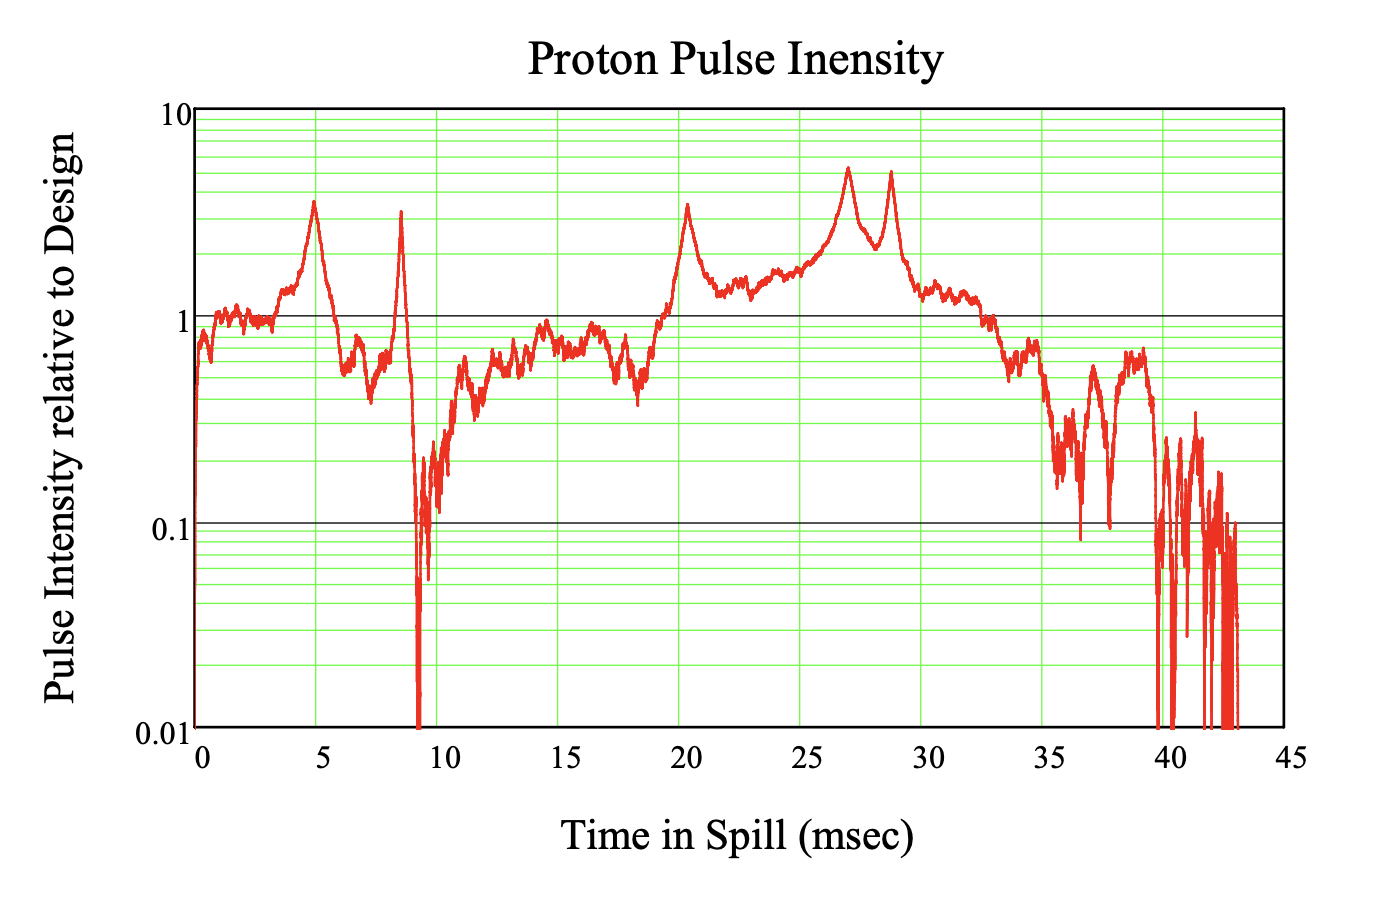
\includegraphics[width=0.8\columnwidth]{figure/Beam intensity.png}
\caption{\textcolor{blue}{\cite{Mu2e_spill} Internal structure of a spill (Beam intensity structure within 45 ms)}. \textcolor{blue}{on the y axis the intensity normalized to the design value.}  For the pulse intensity at 1 can be considered as the I$_0$ after the normalized. Ideally, the beam intensity should be flat at value of 1. However, reality shows that the beam intensity will fluctuate from time to time.}
\label{Bema_intensity}
\end{figure}

\noindent As Figure \ref{Bema_intensity} shows, it is expected to see a large variations of proton pulse intensity, which can affect the detector performance. The variation happens on milliseconds time scale and stopping target monitor (STM) measure the beam flux on a scale of second. Thus it is crucial to monitor the beam fluctuation in milliseconds scale.

\section{Simulation Method and Result}

\begin{figure}[H]
\centering
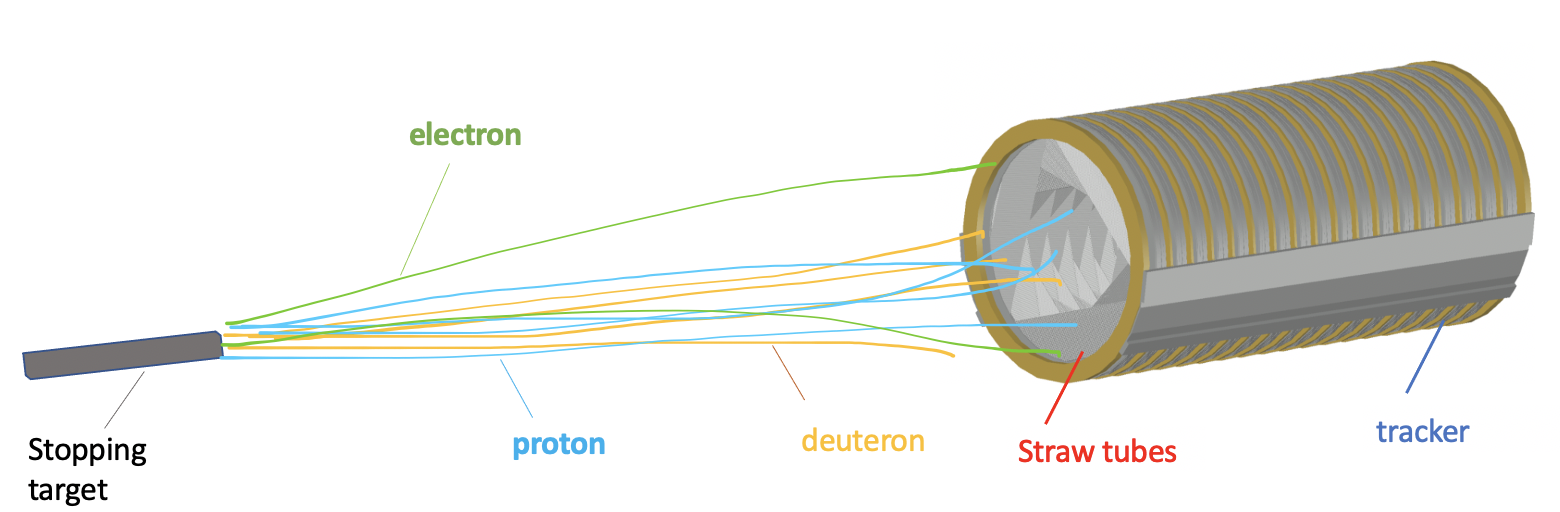
\includegraphics[width=1\linewidth]{figure/simulation.png}
\caption{The schematic of the simulation. There are several assumptions. First, there are only three main particle: electron, deuterium, proton. For single-event simulation, there is a proton/deuterium/electron gun firing at the stopping target.}
\label{}
\end{figure}
\noindent To get the number of the proton in tracker, the single particle simulation is used. In simulation firing the beam gun at the stopping target and assuming the proton, electron and deuterium are the main particle. All situation will be considered into the simulation including the absorb-er effect. 
The goal is to by apply various cut and then try to rule out the electrons and keep the protons number. It is also assumed \textcolor{blue}{(why 'assumed'?)} that a single particle can make number of straw hit and deposit energy in the straw. For simplicity, in the single event simulation, energy of 100MeV electron gun generator is used and the energy distribution for the proton gun will be the shown in figure.
In the mixed event simulation, the energy distribution of the gun generator of the electron and proton will be stimulated as what will be expected in real experiment\cite{Mu2e_Art}. 

\subsubsection{Single Event Simulation }
\begin{figure}[H]
\centering
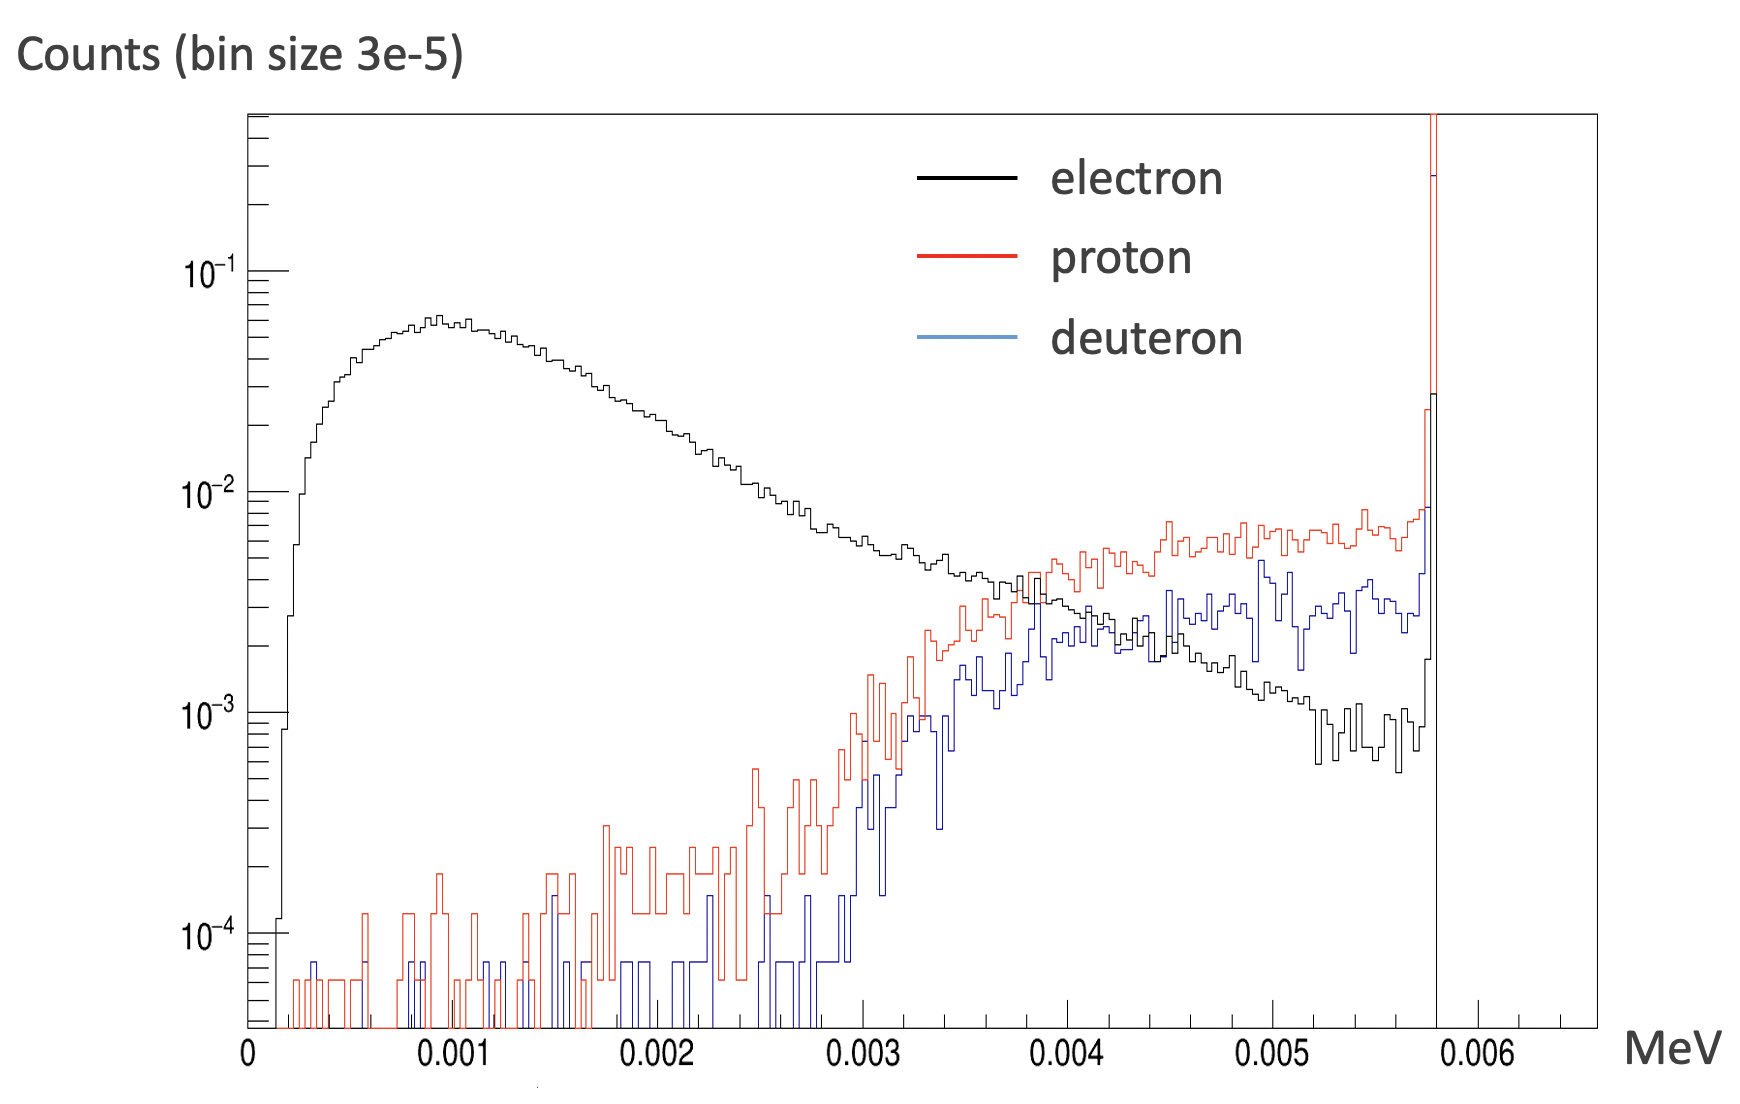
\includegraphics[width=1\linewidth]{figure/qsh_single.png}
\caption{The charge distribution of the electron, proton and deuterium. The red line is the proton and the black line is the electron. The number of electron and proton and deuterium is scaled to the ratio as expected.}
\label{charge}
\end{figure}

\begin{figure}[H]
\centering
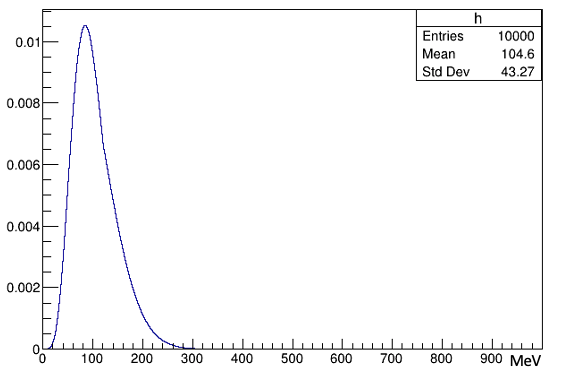
\includegraphics[width=0.9\linewidth]{figure/Generated_proton_p_distribution.png}
\caption{The weighed distribution of momentum of protons which are generated at stopping target. The maximum momentum of proton can go to up to 400MeV.}
\label{generated_proton_p}
\end{figure}

\begin{figure}[H]
\centering
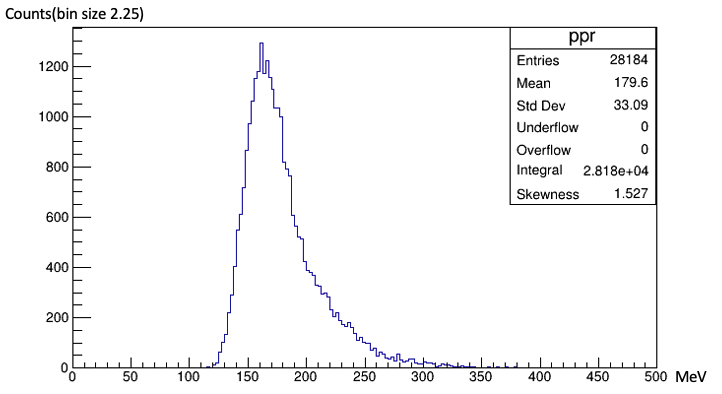
\includegraphics[width=0.9\linewidth]{figure/reconstructed_proton_momentum.png}
\caption{The distribution of momentum of proton which make it through to the tracker. Only protons with momentum 100MeV can make the hit at the tracker.}
\label{proton_P}
\end{figure}

\noindent In order to lower the number of electron and keep the number of proton as much as possible, it is easily found that making the cut of charge around 0.004 MeV as shown in figure\ref{charge} can reach the goal.


\begin{figure}[H]
\centering
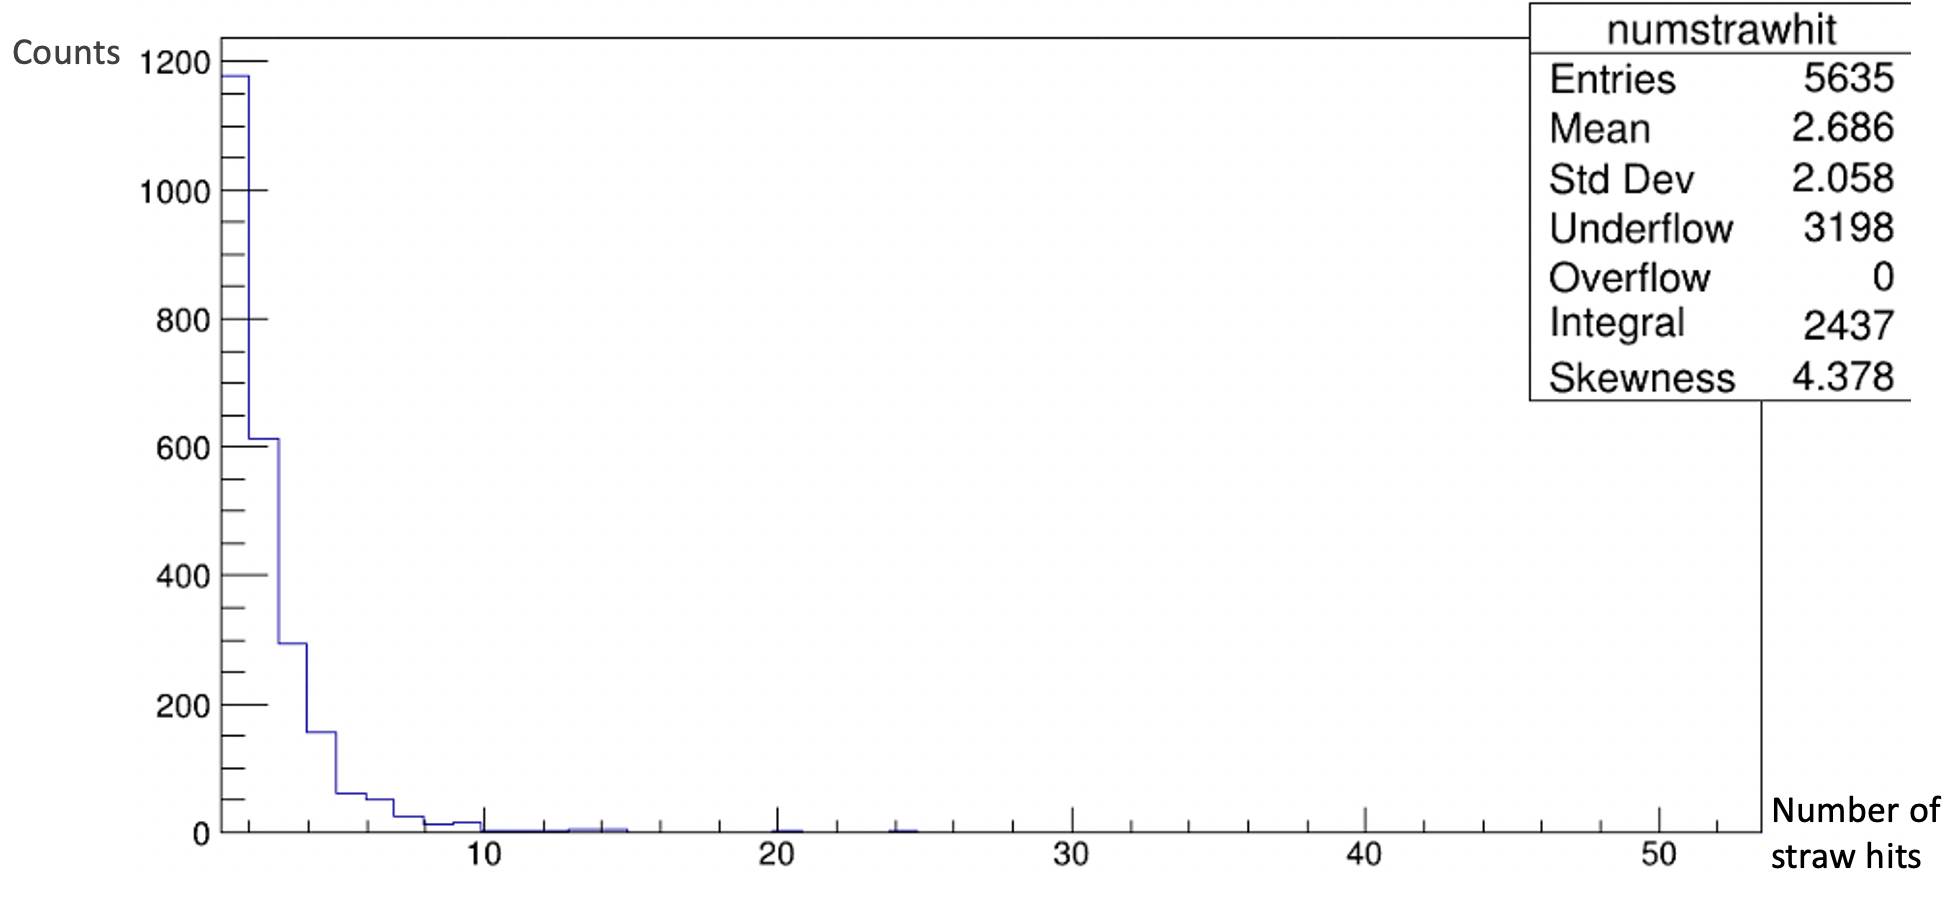
\includegraphics[width=0.9\linewidth]{figure/electron_sh.png}
\caption{The distribution of number of straw hit that made by the electron after applying the cut of charge cut at 0.004 MeV.The plot is generated by 10k event of single event of electron.}
\label{electron_sh}
\end{figure}


\begin{figure}[H]
\centering
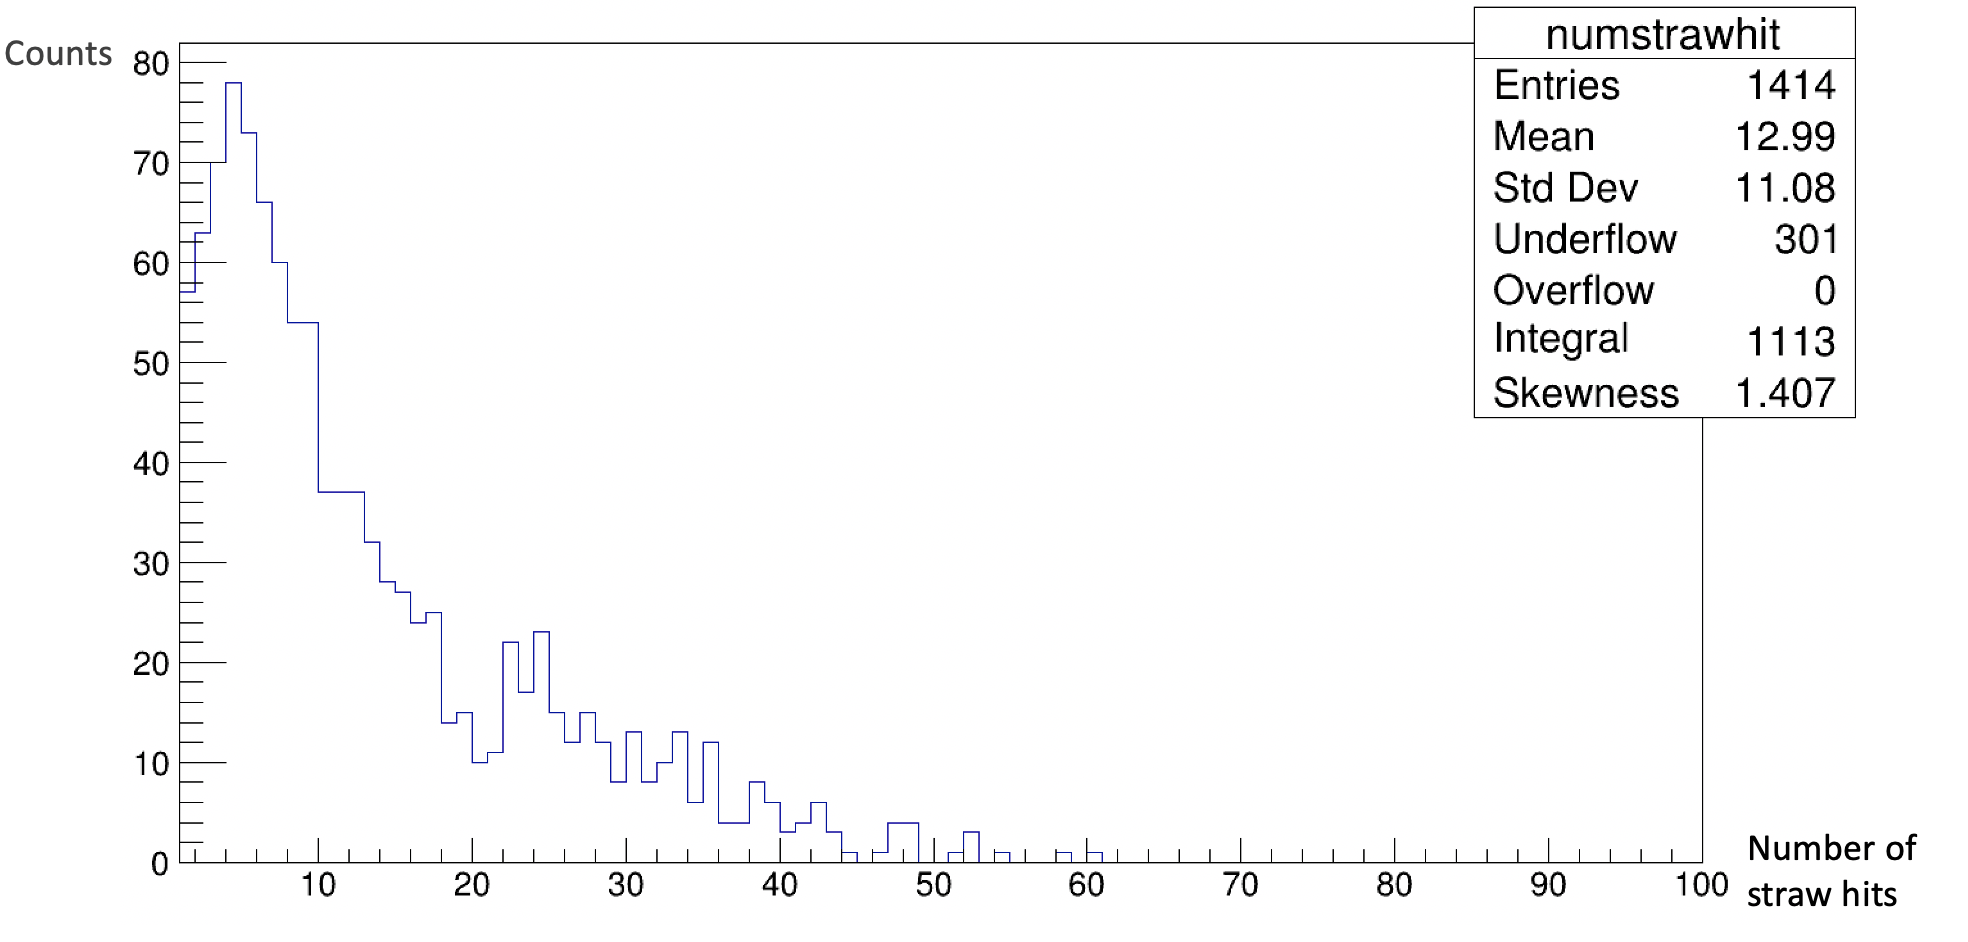
\includegraphics[width=0.9\linewidth]{figure/proton_sh.png}
\caption{The distribution of number of straw hit that made by the proton after applying the cut of charge cut at 0.004 MeV. The plot is generated by 100k event of single event of proton.}
\label{proton_sh}
\end{figure}
\noindent After comparing Figure \ref{electron_sh} with Figure \ref{proton_sh}, it can be concluded that making the cut at straw hit number of 10 can reduce most of number of electron and keep most of proton. 

\subsubsection{Mixed Event Simulation }

\begin{figure}[H]
\centering
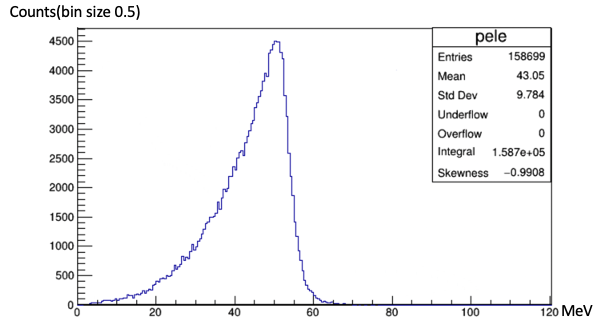
\includegraphics[width=1\linewidth]{figure/reconstructed_electron_momentum.png}
\caption{The distribution of momentum of electron which make it through the tracker.}
\label{generated_e_p}
\end{figure}

\begin{figure}[H]
\centering
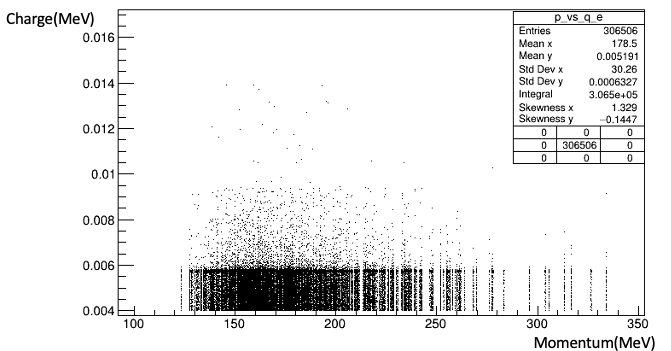
\includegraphics[width=1\linewidth]{figure/Momentum_electron_charge.png}
\caption{The charge distribution of electron with respect to the momentum of electron. The 0.004MeV charge cut-off is due to the charge cut.}
\label{generated_e_p_Q}
\end{figure}


\begin{figure}[H]
\centering
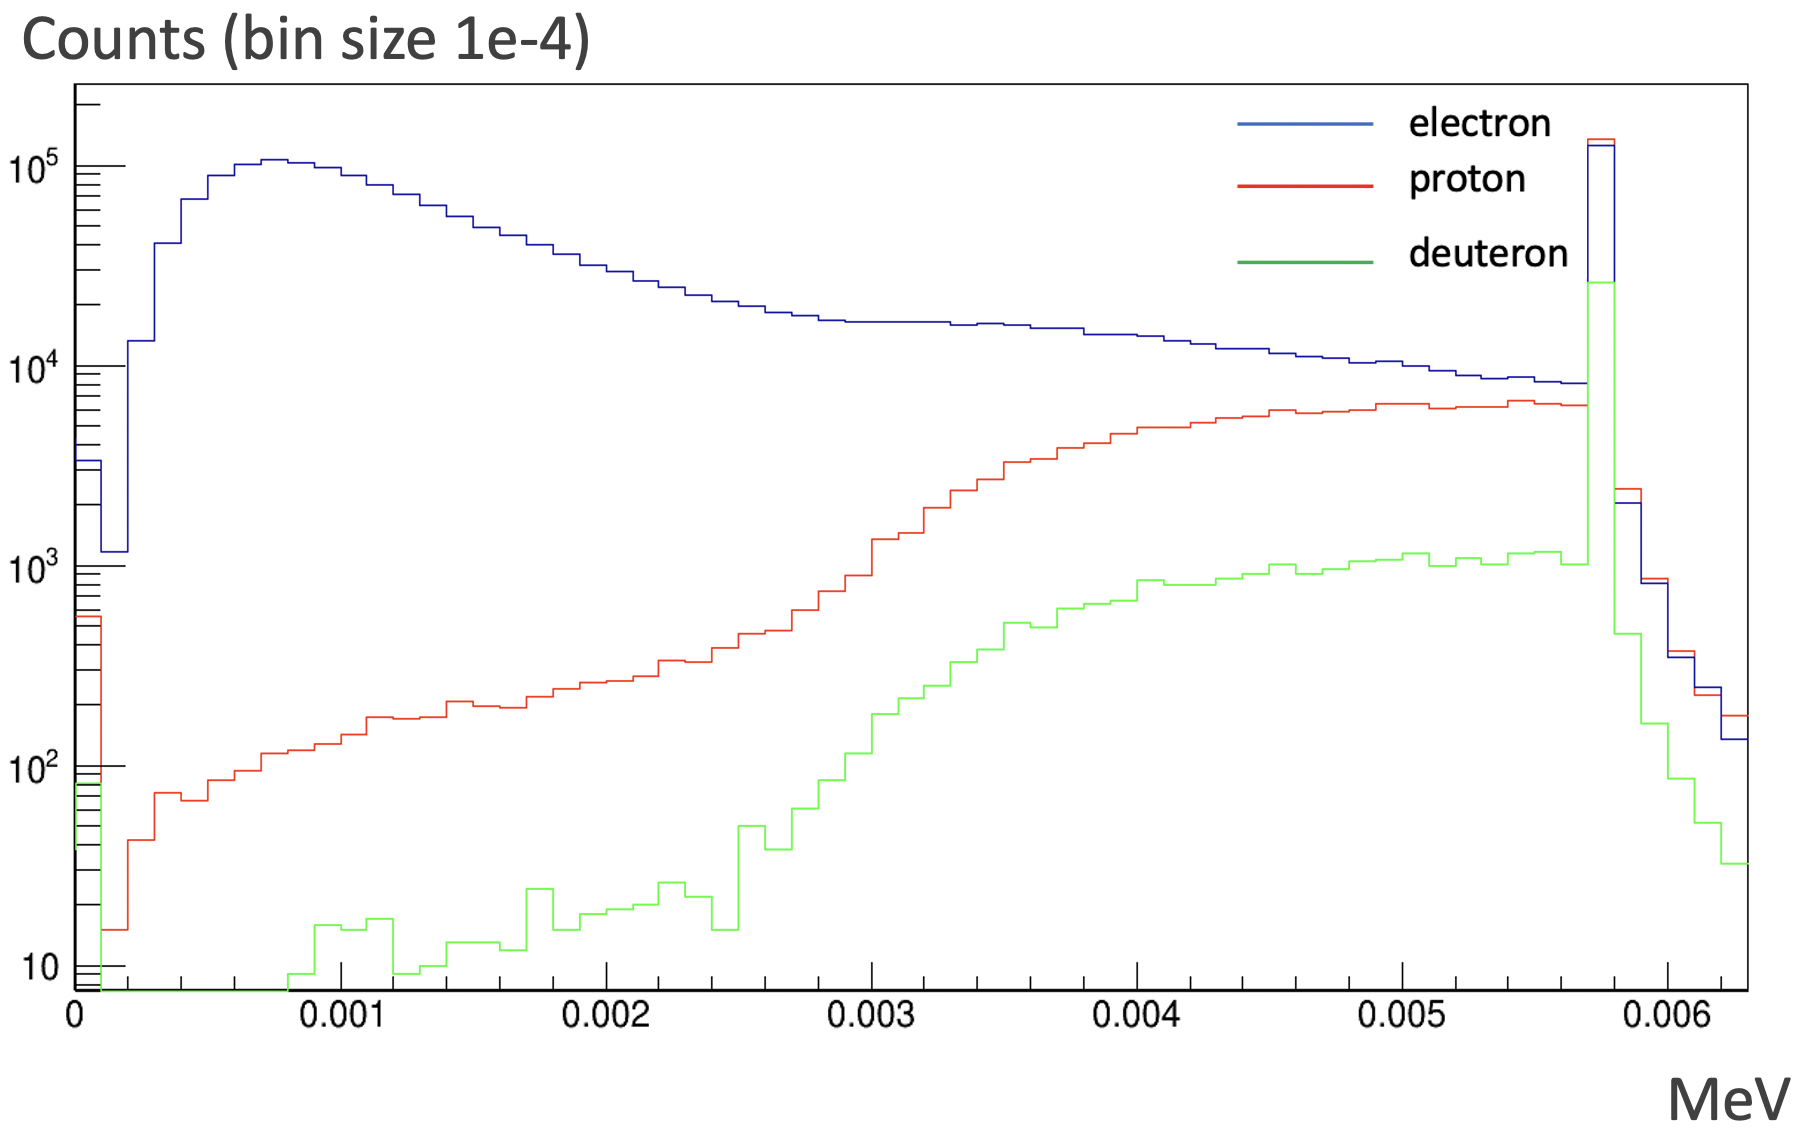
\includegraphics[width=0.9\linewidth]{figure/qsh_mixed.png}
\caption{The distribution of charge for each particle in mixed event in log scale.}
\label{charge2}
\end{figure}
\noindent 
By comparing with the Figure\ref{charge}, we can see there is longer tail for electron in Figure\ref{charge2}. It is because in the single particle simulation, only 100MeV electrons are considered. In the Mixed particle event, the energy distribution of electron is closer to the real situation. There is more low momentum electron and these low momentum electrons cause the long tail in electron charge distribution. It is also showing the proton and deuteron are minority. But still, making the cut at 4keV of the charge can increase the ratio of the proton number over the electron number.





\begin{figure}[H]
\centering
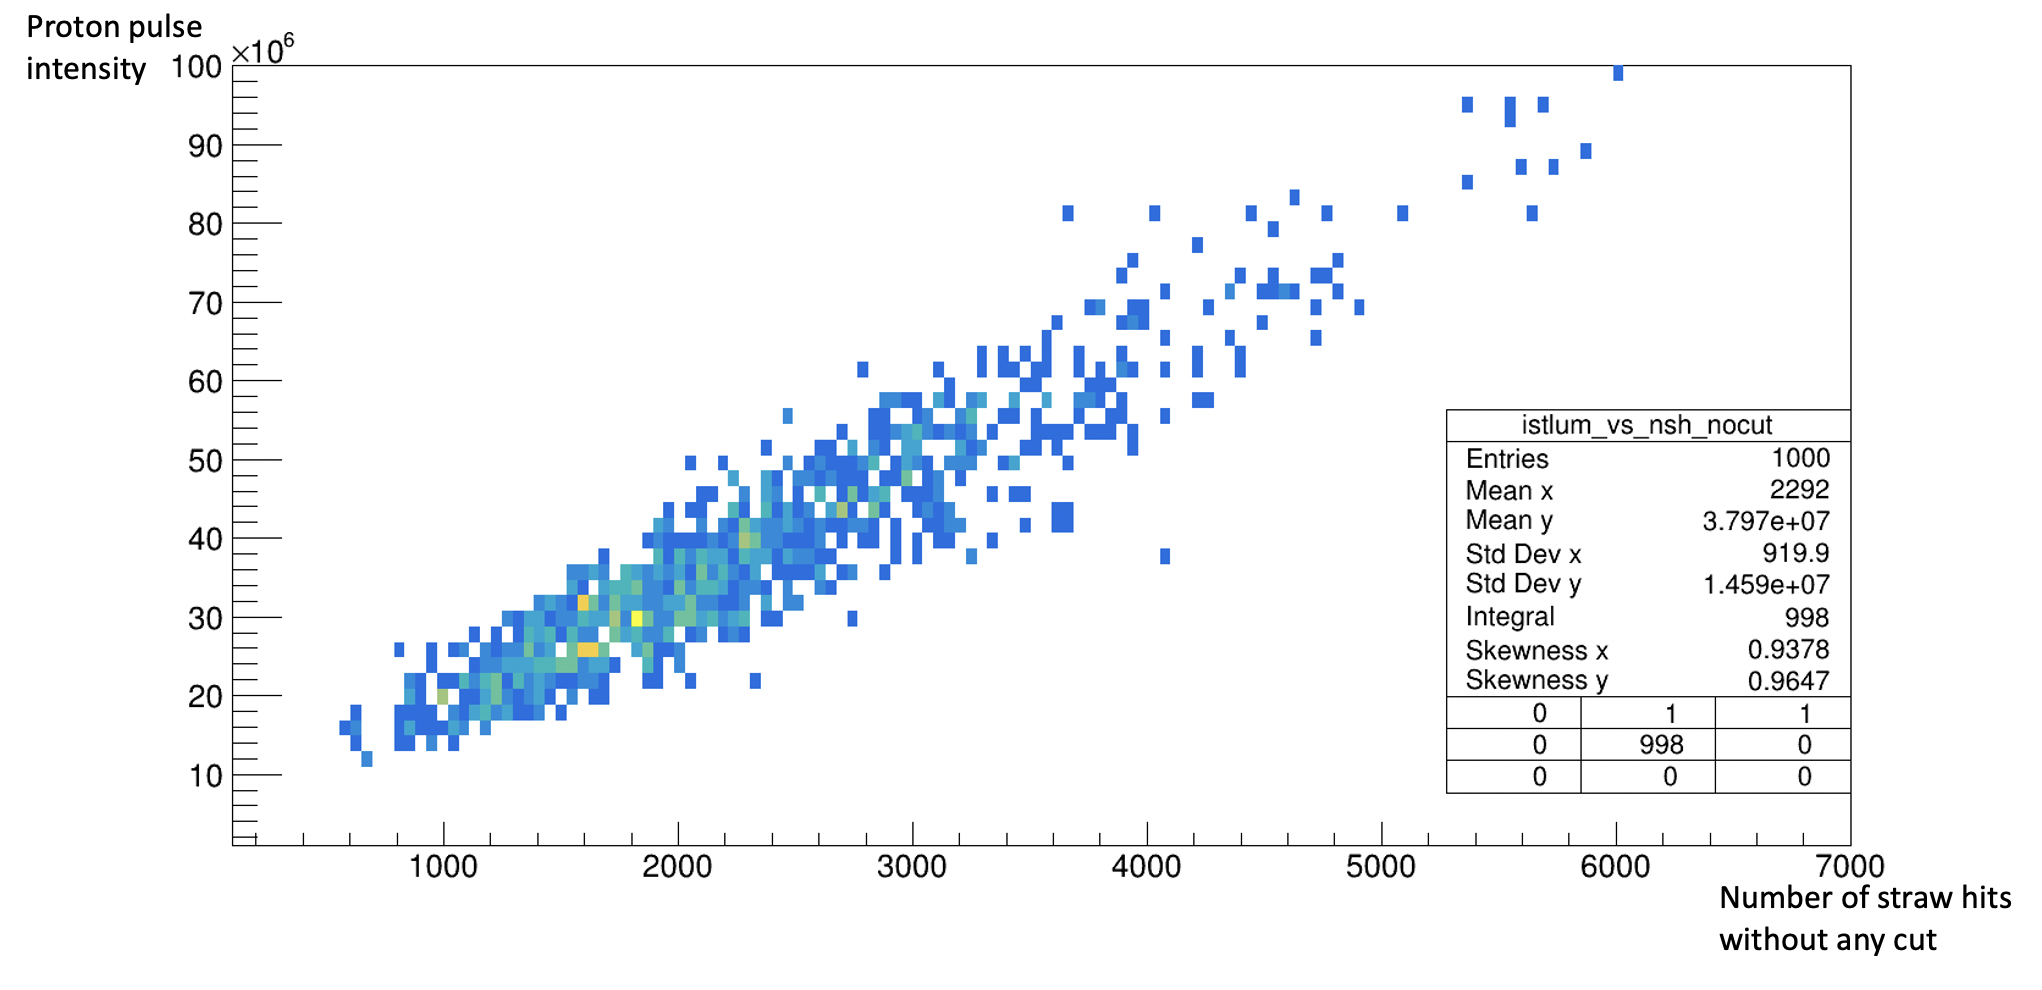
\includegraphics[width=1.1\linewidth]{figure/Lum_vs_hits_png.png}
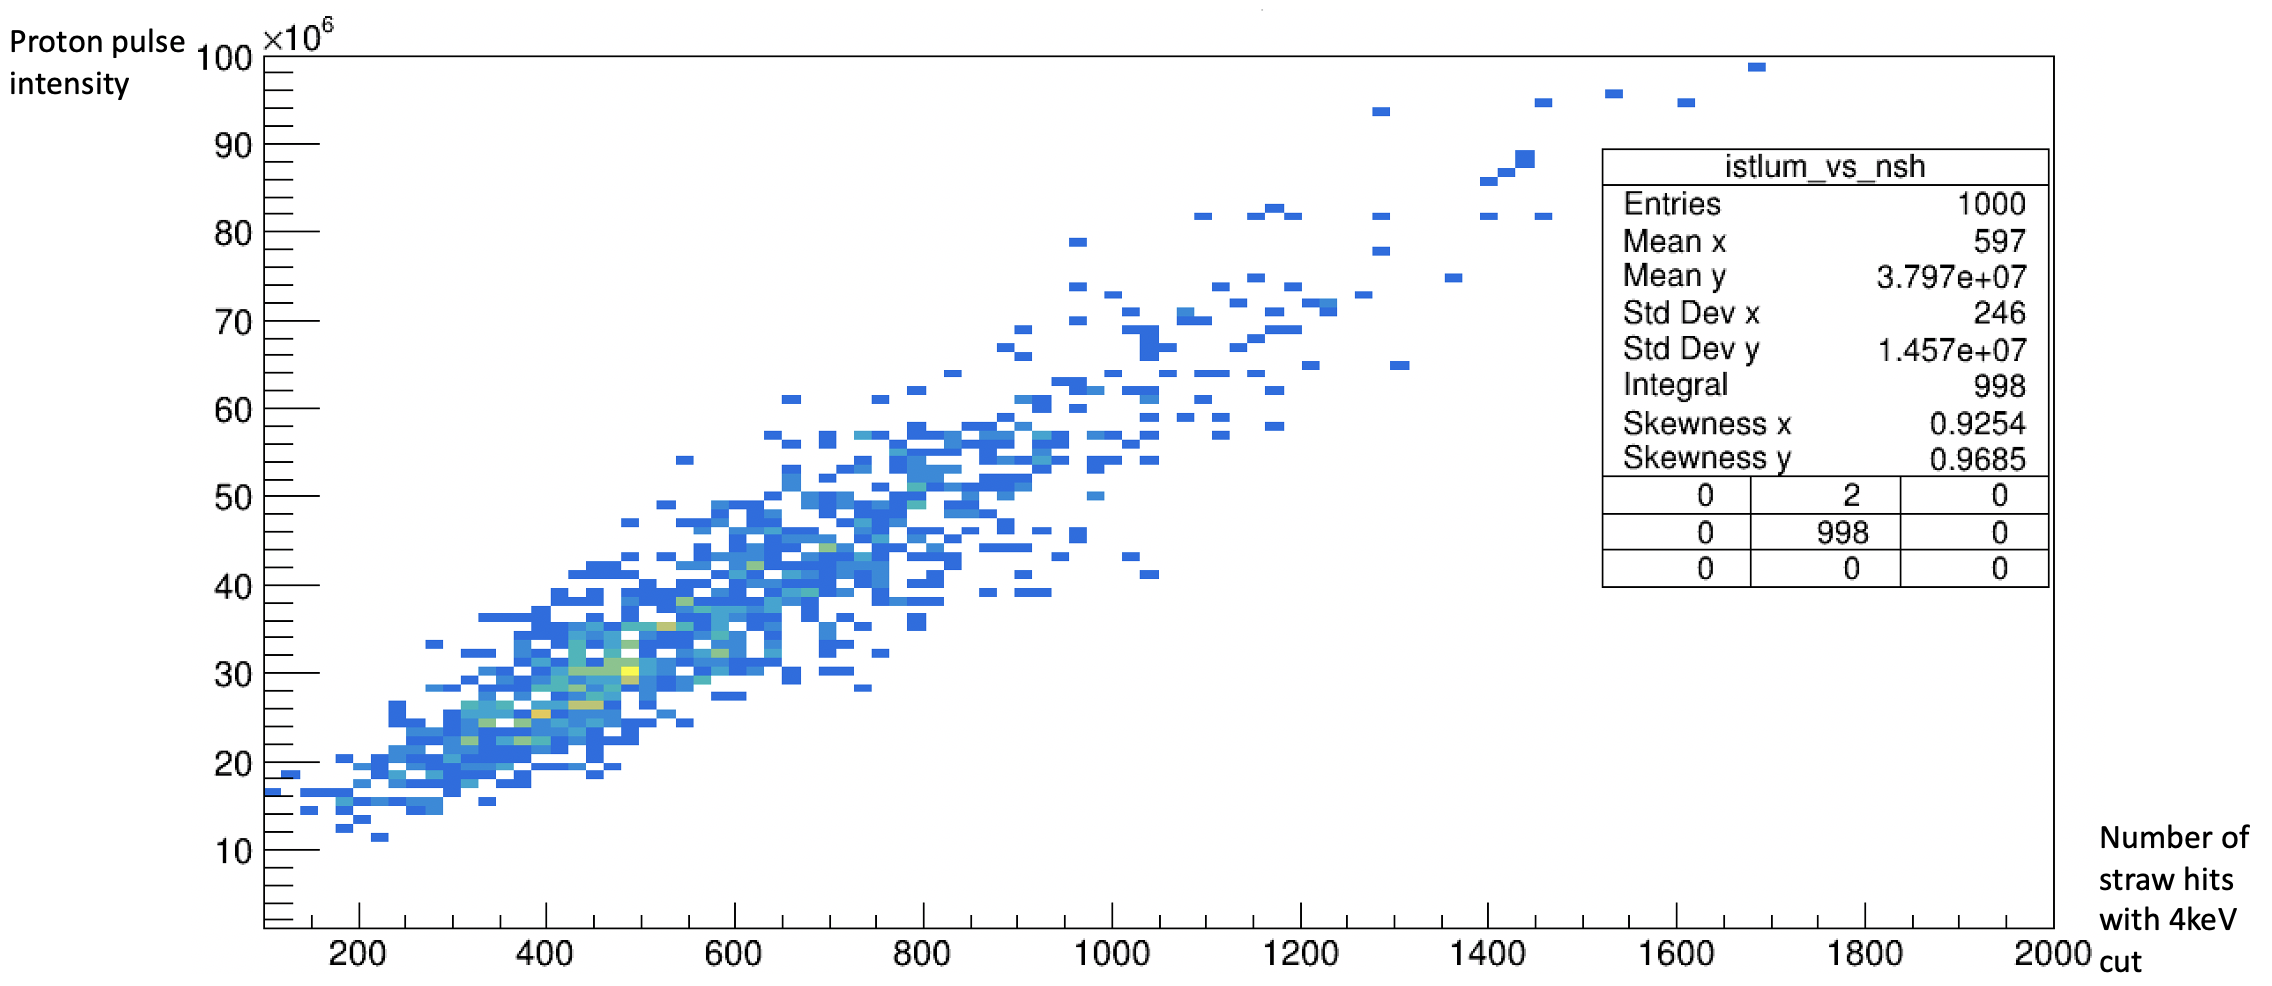
\includegraphics[width=1.1\linewidth]{figure/Lum_vs_protonhits.png}
\caption{The top one is the proton pulse intensity verse the total of the straw hits without applying any cut and the bottom one is the proton pulse intensity verse number of the straw hits with the cut of 4keV }
\label{Lum_vs_totalhits}
\end{figure}
\noindent It can be seen that the number of hits is almost proportional to the beam intensity. However, it is impossible to tell how many portion of the hits are due to the muon stopped target. There are lot of processes contributing to there hits which has nothing to do with the stopped muon rate. So the rest of the goal is to eliminate the portion of these hits which is not related with the process of the muon stopped target. 
There is great temptation to count the proton since proton come from the stopping target. The main goal becomes how to make sure the hit are from the proton from the stopping target.


\begin{figure}[H]
\centering
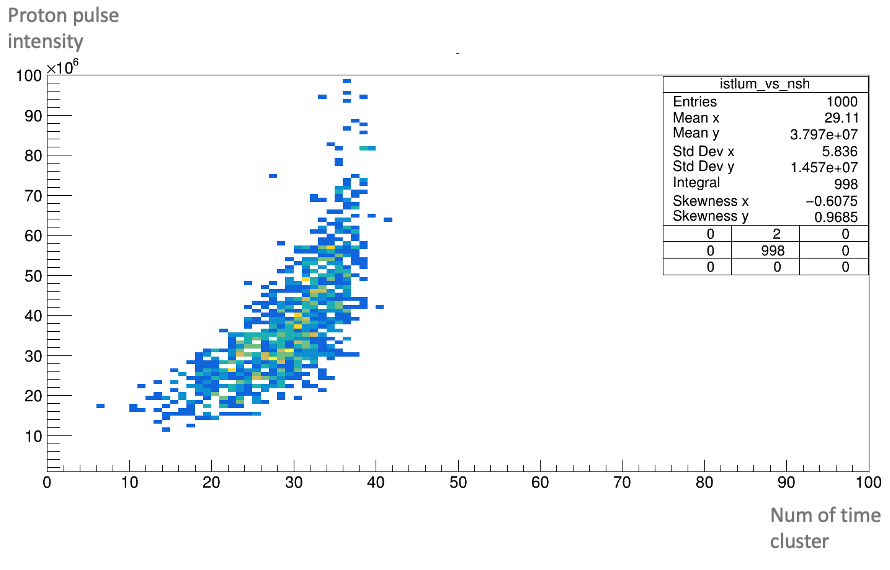
\includegraphics[width=0.8\linewidth]{figure/Lum_vs_timecluster_nocut.png}
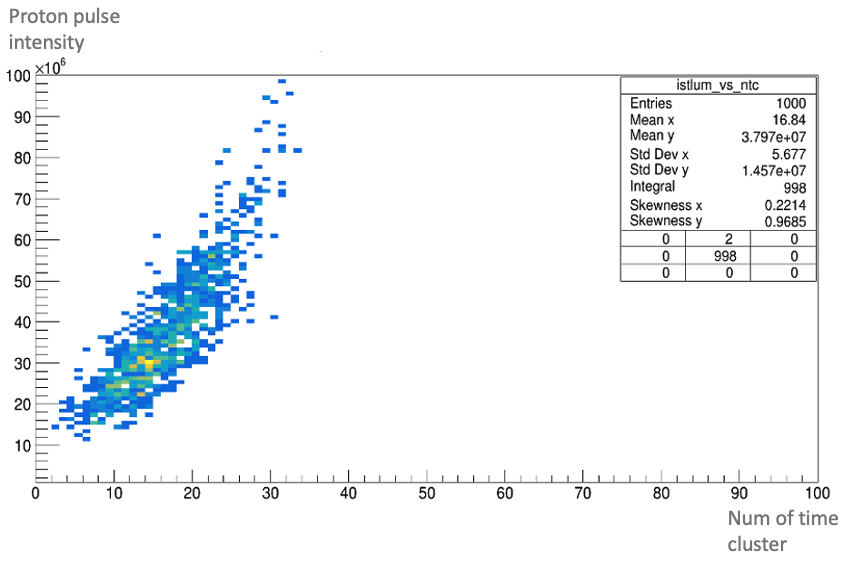
\includegraphics[width=0.79\linewidth]{figure/Lum_vs_timecluster_cutQ.png}
\caption{The proton pulse intensity verse the number of time clusters.The top one of Figure \ref{Lum_vs_tc} is the time cluster without the 4 keV charge cut within microbunch. The bottom one is the time cluster with the 4 keV charge cut within microbunch}
\label{Lum_vs_tc}
\end{figure}
\noindent 
When using the number of time cluster to monitor the stopped muon rate, the next question will be, how many time cluster are made by background, for example, the proton coming from the outside of the stopping target.
Also the ratio of time clusters made by the background over the time clusters made by the proton from the stopping target. In the next section, it would explore about this ratio.


\subsubsection{Background Simulation}

\begin{figure}[H]
\centering
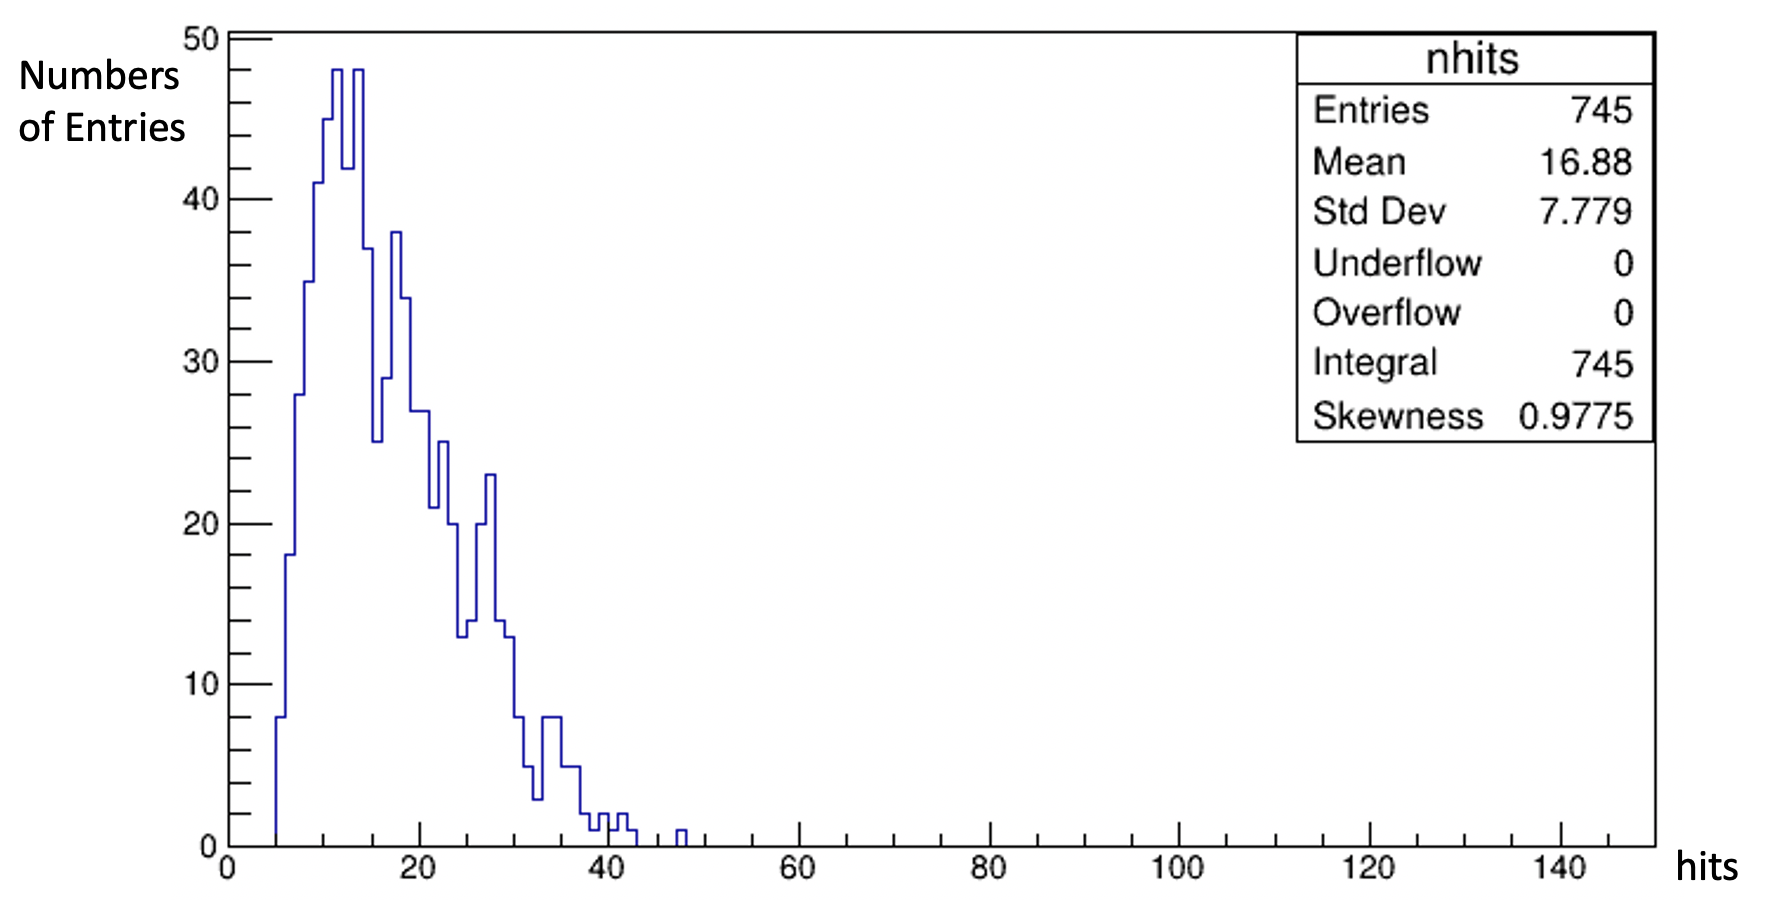
\includegraphics[width=0.8\linewidth]{figure/proton_oot_timecluster.png}
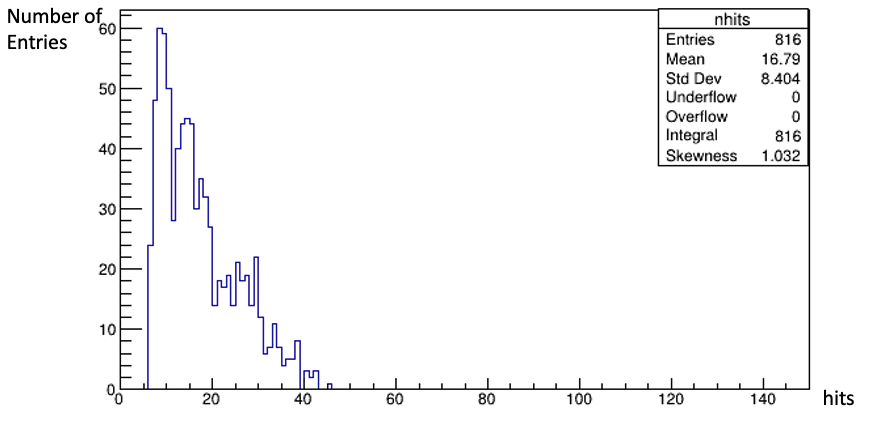
\includegraphics[width=0.81\linewidth]{figure/proton_stopped_target_timecluster.png}
\caption{The top one of Figure \ref{timecluster} shows that the number of hits distribution made by proton coming from outside of the stopping target and the bottom one of Figure \ref{timecluster} is number of proton from stopping target. The difference between the proton coming from outside of the stopping target and from stopping target is small.
}
\label{timecluster}
\end{figure}
\noindent 

\noindent For single proton event coming from the stopping target, with 10$^5$ events generated, there will be 1414 events could pass through the tracker. For the proton coming from outside of the stopping target, with 5x10$^7$ events generated, only 1243 events pass through the tracker. Thus the acceptance ratio of the proton coming from stopping target over the proton coming from outside of the stopping target is order of 2:
 \[   
 \frac{ 1243 }{ 5\times10^{7}}= 2.5\times10^{-5}
\]
\[
     \frac{ 1414 }{10^{5}} = 1.4\times10^{-2}
\]

\[
     \frac{ 1.4\times10^{-2} }{ 2.5\times10^{-5}} = 5\times10^{2} 
\]


\\Also the background coming from outside of stopping target  is less than 1 \%. \\
\\It can be concluded that measuring the muon flux stopped on target by counting the proton in the tracker.







\section{Analysis}
The goal for counting of number of proton is to monitor the fluctuation of the proton beam intensity. Not only the statistical uncertainty of the counting proton number can be reached to $\sim$1\% in milliseconds scale, but also the change of the efficiency of the counting the proton number is quite stable under the change of the beam fluctuation.
\noindent The number of proton per micro-bunch in full luminosity after reconstruction will be around: 
\[ 3.9 \times 10 ^7 \times 1.6 \times 10^{-3} \times 0.6 \times 0.035 \times 0.006  = 8 \]
Where the 3.9 x $10^{7}$ is the the proton at production target per micro-bunch, 
1.6 x $10^{-3}$ is the probability per proton of muon stopping per micro-bunch, 
0.6 is the probability of muon nuclear capture, 0.0035 is the probability of generated proton from nuclear capture, and 0.006 is the efficiency of the reconstructing the proton by the way of applying the charge cut and the straw hits above 10 cut. There are $\sim$590 pulses in one millisecond, thus statistical uncertainty of the counting proton number:
\[
     \frac{ \sqrt{590 \times 8}  }{ 590 \times 8} = 1 \%
\]
\noindent With more information on the fluctuation, we can estimate the normalization factor better.

\begin{table}[!h]
\centering
\begin{tabular}{llll}
Error & Required Time   \\
10\%    &  0.02 milliseconds \\
1\%     &  1 millisecond   \\
\end{tabular}
\caption{Error of counting proton number and corresponding time}
\label{equip1}
\end{table}






\begin{thebibliography}{9}


\bibitem{Intro_STM} 
Introduction to STM Document 34650-v2
\\\texttt{https://mu2e-docdb.fnal.gov/cgi-bin/private/RetrieveFile?docid=34650&filename=miller-review-intro-STM-vf.pdf&version=2}

\bibitem{STM_baseline} 
STM baseline design 6453-v4
\\\texttt{https://mu2e-docdb.fnal.gov/cgi-bin/private/RetrieveFile?docid=6453&filename=stm\_design\_memo.pdf&version=4}

\bibitem{P_Generated_proton} 
Charged-particle spectra from \Pmuon capture on Al
\\\texttt{https://arxiv.org/pdf/1908.06902.pdf}

\bibitem{Bastiano_reco} 
Mu2e Document 36048-v1
\\\texttt{https://mu2e-docdb.fnal.gov/cgi-bin/private/ShowDocument?docid=36048}


\bibitem{Mu2e_proposal} 
Mu2e proposal
\\\texttt{https://mu2e-docdb.fnal.gov/cgi-bin/ShowDocument?docid=388}

\bibitem{Mu2e_spill} 

Mu2e Document 33344-v3
\\\texttt{https://mu2e-docdb.fnal.gov/cgi-bin/private/ShowDocument?docid=33344}

\bibitem{Mu2e_Art} 
Running art
\\\texttt{https://mu2ewiki.fnal.gov/wiki/Running_Art_Tutorial}

\bibitem{Mu2e_Jobsubmit} 
Submit Job on Mu2e grid
\\\texttt{https://mu2ewiki.fnal.gov/wiki/SubmitJobs}






\end{thebibliography}
\end{document}
